\documentclass{article}

%
% 引入模板的style文件
%
\usepackage{homework}

\setCJKmainfont{SimSun}[AutoFakeBold] %宋体加粗
\setCJKsansfont{SimHei}[AutoFakeBold] %黑体加粗


\usepackage{minted} %配合minted宏包进行好看的高亮
\usepackage{currfile} %配合minted宏包进行好看的高亮
\usepackage{caption} %配合minted宏包进行好看的高亮
\usepackage{tcolorbox} %配合minted宏包进行好看的高亮
\usepackage{xcolor} %配合minted宏包进行好看的高亮
\tcbuselibrary{skins} %配合minted宏包进行好看的高亮
\tcbuselibrary{minted} %配合minted宏包进行好看的高亮
\usemintedstyle{paraiso-dark} %配合minted宏包进行好看的高亮
\usepackage{framed} 
\usepackage{amsmath}


%
% 封面
%


\title{
	
\includegraphics[width=0.6\textwidth]{images/title/ucas_logo 1.pdf}\\
    \vspace{1in}
    \textmd{\textbf{\hmwkClass}}\\
	\textmd{\Large{\textbf{\hmwkClassID}}}\\
    \textmd{\textbf{\hmwkTitle}}\\
    \normalsize\vspace{0.1in}\large{\hmwkCompleteTime }\\
    \vspace{0.1in}\large{\textit{\hmwkClassInstructor\ }}\\
    \vspace{1in}
	
\includegraphics[width=0.25\textwidth]{images/title/Cyber.jpg}\\
	\vspace{1in}
}

\author{
	\hmwkAuthorName \\ 
	\hmwkAuthorStuID \\
	\hmwkAuthorInst \\
	\hmwkAuthorzhuanye \\
	\hmwkAuthorfangxiang
	}
\date{}

\renewcommand{\part}[1]{\textbf{\large Part \Alph{partCounter}}\stepcounter{partCounter}\\}


%
% 正文部分
%
\begin{document}


\maketitle


%\include{chapters/ch01}
%\include{chapters/ch02}
%\include{chapters/ch03}
%\include{chapters/ch04}
%\include{chapters/ch05}


\pagebreak



\begin{homeworkProblem}
	最大子段和问题: 给定整数序列$a_1, a_2, \cdots, a_n$, 求该序列形如$\displaystyle \sum_{k=i}^j a_k$的子段和的最大值: $$\displaystyle \text{max} \left\{0, \underset{1\le i\le i\le n}{\text{max}} \sum_{k=i}^j a_k\right\}$$
	
	(1). 已知一个简单算法如下:
\begin{tcblisting}{listing engine=minted,boxrule=0.1mm,
colback=blue!5!white,colframe=blue!75!black,
listing only,left=5mm,enhanced,sharp corners=all,
overlay={\begin{tcbclipinterior}\fill[red!20!blue!20!white] (frame.south west)
rectangle ([xshift=5mm]frame.north west);\end{tcbclipinterior}},
minted language=c++,
minted style=tango,
minted options={fontsize=\small,breaklines,autogobble,linenos,numbersep=3mm}}
int Maxsum(int n, vector<int> a, int& besti, int& bestj) {
    int sum = 0;
    for(int i = 1; i <= n; i++) {
        int suma = 0;
        for(int j = i; j <= n; j++) {
            suma += a[j];
            if(suma > sum) {
                sum = suma;
                besti = i;
                bestj = j;
            }
        }
    }
    return sum;
}
\end{tcblisting}
	试分析该算法的时间复杂性;

	(2). 试用分治算法解最大子段和问题, 并分析算法的时间复杂性;

	(3). 试说明最大子段和问题具有最优子结构性质, 并设计一个动态规划算法求解最大子段和问题, 分析算法的时间复杂度. (提示: 可令$\displaystyle b\left( j \right) =\underset{1\le i\le j\le n}{\text{max}}\sum_{k=i}^j{a_k}, j=1,2,\cdots ,n$)
	\\

	\solution \,\,(1). 显然第2层for循环里面的操作都是常数次的(记为$C$), 所以算法总的关键操作数为$$\sum_{i=1}^n{\sum_{j=i}^n{C}}=C\sum_{i=1}^n{\left( n-i+1 \right)}=\frac{1}{2}C\left( n^2+n \right) 
	$$
	故显然时间复杂度为$T(n)=O(n^2)$.

	(2). 采用分治算法, 则考虑: 先将数组从中间mid切开. 此时, 最大和的子段可能出现在左半边, 也可能出现在右半边, 也有可能横跨左右两个子数组. 所以需要返回这三种情况下所分别对应的子问题解的最大值. 

	当最大和的子段出现在左半边(右半边同理)时, 继续分中点递归直至分解到只有一个数为止;

	当最大和的子段横跨mid左右时, 只需分别求解左子数组的最优后缀和以及右子数组的最优前缀和. 这三种情形下的最大值即为整个数组的最大子段和. 具体分治算法见如下.
	\begin{algorithm}[H]
		\begin{algorithmic}[1]
		\Require{数组$A$, 左边界left, 右边界right}
		\Ensure{$A$的最大子段和sum及子段的前后边界}
		\If{left==right}
			\State \Return max($A$[left], 0);
		\EndIf
		\State $k:=$(left+right)/2;
		\State leftsum $=$ \textbf{MaxSubSum}($A$,left,$k$);
		\State rightsum $=$ \textbf{MaxSubSum}($A$, $k+1$,right);
		\State 类似(1)中的算法分别求得$S_1,S_2$;
		\State Sum$:=S_1+S_2$;
		\State \Return max(leftsum, rightsum, Sum);
		\State \textbf{end \{MaxSubSum\}}
		\end{algorithmic}
		\caption{\textbf{MaxSubSum}($A$, left, right)}
		\label{alg:MaxSubSum}
	\end{algorithm}
	
	可以看出最坏情形下的时间复杂度的递推式和结果分别为$T\left( n \right) =2T\left( \frac{n}{2} \right) +O\left( n \right)
	$, 故根据主定理($\log_b(a)=\log_2(2)=1=d$)可知$T(n)=O(n\log n)$.
	

	(3). 先证明此问题具有最优子结构性质: 依次考虑($1\leq i\leq n$)以$a[i]$\textbf{为结尾}的最大子段和$C[i]$, 然后在这$n$个值当中取最大值即为原问题答案. 假设以$a[i]$为结尾的最大(和)子段为$\{a[k],\cdots,a[i]\}$, 那么$\{a[k],\cdots,a[i-1]\}$一定是以$a[i-1]$为结尾的最大(和)子段. 否则若$\{a[m],\cdots,a[i-1]\}$为以$a[i-1]$为结尾的最大(和)子段, 那么$\{a[m],\cdots,a[i-1],a[i]\}$就是以$a[i]$为结尾的最大(和)子段, 这显然与假设相矛盾, 也就是说该优化函数是满足优化原则的(即此问题具有最优子结构性质). 

	现在来推导$C[i]$的递推表达式: 当$C[i-1]\leq 0$, 说明$C[i-1]$对应的子段对于整体的贡献是没有的, 所以$C[i]\gets a[i]$; 当$C[i-1]>0$, 说明$C[i-1]$对应的子段对于整体的是有贡献的, 于是$C[i]\gets a[i]+C[i-1]$. 两种可能情况(对应两种决策)取最大值即可:$$\begin{cases}
		C\left[ i \right] =\text{max} \left\{ a\left[ i \right] ,C\left[ i-1 \right] +a\left[ i \right] \right\} , 2\le i\le n\\
		C\left[ 1 \right] =a\left[ 1 \right]\\
	\end{cases}
	$$
	最后返回数组$C$中的最大值($\displaystyle \underset{1\le i\le n}{\text{max}}C\left[ i \right] $)即可. 计算$C[i]$的过程需要消耗$O(n)$的时间, 找出数组最大值也需要$O(n)$的时间(一次遍历), 所以算法的总时间复杂度为$T(n)=O(n)$. 并且我们可以给出C++代码:
\begin{tcblisting}{listing engine=minted,boxrule=0.1mm,
colback=blue!5!white,colframe=blue!75!black,
listing only,left=5mm,enhanced,sharp corners=all,
overlay={\begin{tcbclipinterior}\fill[red!20!blue!20!white] (frame.south west)
rectangle ([xshift=5mm]frame.north west);\end{tcbclipinterior}},
minted language=c++,
minted style=tango,
minted options={fontsize=\small,breaklines,autogobble,linenos,numbersep=3mm}}
int mostvalue(vector<int>& a) { //时间复杂度为O(n), 空间复杂度为O(n)
    int n = a.size();
    vector<int> dp(n);
    dp[0] = a[0];
    for(int i = 1; i < n; i++) {
        dp[i] = max(dp[i - 1] + a[i], a[i]);
    }
    int index = max_element(dp.begin(), dp.end()) - dp.begin();
    return dp[index];
}
\end{tcblisting}
\end{homeworkProblem}


\pagebreak

\begin{homeworkProblem}
	设$A=\left\{ x_1,x_2,\cdots ,x_n \right\} $是$n$个不等的整数构成的序列, $A$的一个单调递增子序列是指序列$\{ x_{i_1},x_{i_2},$
	$\cdots ,x_{i_k} \} ,i_1<i_2<\cdots i_k	$且$x_{i_1}<x_{i_2}<\cdots <x_{i_k}$.(子序列包含$k$个整数). 例如, $A=\left\{ 1,5,3,8,10,6,4,9 \right\} $, 他的长度为4的递增子序列是: $\left\{ 1,5,8,10 \right\} ,\left\{ 1,5,8,9 \right\} ,\cdots$.设计一个算法, 求$A$的最长的单调递增子序列, 分析算法的时间复杂度. 对于输入实例$A=\left\{ 2,8,4,-4,5,9,11 \right\} $, 给出算法的计算过程和最后的解.
	\\

	\solution 定义$dp[i]$是以$\text{nums}[i]$\textbf{为结尾}(且考虑前$i$个元素)的最长单增子序列的长度. 于是可以写出如下转移方程$(i\geq 1)$和初始条件:
    $$
    dp\left[ i \right] =\left\{ \begin{matrix}
        \underset{0\le j\le i-1}{\text{max}}dp\left[ j \right] +1,&		\exists j\in \left[ 0,i-1 \right] , s.t. \,\text{nums}\left[ j \right] <\text{nums}\left[ i \right]\\
        1&		\forall j\in \left[ 0,i-1 \right] , s.t. \,\text{nums}\left[ j \right] >\text{nums}\left[ i \right]\\
    \end{matrix} \right. , dp\left[ 0 \right] =1
    $$
    显然, 若$dp[i]$的子序列是$i_1i_2\cdots i_ki$, 则$dp[i_k]$的子序列为$i_1i_2\cdots i_k$, 即问题满足最优子结构性质. 需借助数组$m$来对解进行回溯(即$m[i]$记录$dp[i]$是由哪个下标的状态转移而来的). 而要想算出\textbf{整个数组}的最长单增子序列长度, 则需要算好所有的$dp[i]$值, 再对$dp$数组进行遍历, 由此得到最长单增子序列长度和对应下标. 最后使用数组$m$进行回溯以取得答案. 可以看出, 算法的空间复杂度为$O(n)$, 而时间复杂度显然为$$T\left( n \right) =O\left( \sum_{i=0}^{n-1}{\sum_{j=0}^{i-1}{1}} \right) =O\left( \sum_{i=0}^{n-1}{i} \right) =O\left( \frac{n\left( n-1 \right)}{2} \right) =O\left( n^2 \right) 
	$$
	我们将上述的最优值求解过程和解的回溯过程写成C++代码, 并且已完全通过\href{https://leetcode.cn/problems/longest-increasing-subsequence/description/}{\textbf{LeetCode-T300}}的所有测试样例, 具体如下所示:
\begin{tcblisting}{listing engine=minted,boxrule=0.1mm,
colback=blue!5!white,colframe=blue!75!black,
listing only,left=5mm,enhanced,sharp corners=all,
overlay={\begin{tcbclipinterior}\fill[red!20!blue!20!white] (frame.south west)
rectangle ([xshift=5mm]frame.north west);\end{tcbclipinterior}},
minted language=c++,
minted style=tango,
minted options={fontsize=\small,breaklines,autogobble,linenos,numbersep=3mm}}
vector<int> LIS(vector<int>& nums) {
    int n = nums.size();
    vector<int> dp(n, 0);
    dp[0] = 1;
    vector<int> m(n, 0); 
    for (int i = 1; i <= n - 1; i++) {
        int prev = i, len = 1; 
        for (int j = 0; j <= i - 1; j++) {
            if (nums[j] < nums[i]) { 
                if (dp[j] + 1 > len) {
                    len = dp[j] + 1;
                    prev = j;
                }
            }
        }
        dp[i] = len, m[i] = prev; 
    }
    int index = max_element(dp.begin(), dp.end()) - dp.begin(); 
    int MaxLen = dp[index]; 
    vector<int> res;
    while (res.size() != MaxLen) {
        res.push_back(nums[index]);
        index = m[index];
    }
    return res;
}
\end{tcblisting}

	对于具体实例, 计算过程如下:
	\begin{align}
		&C\left[ 1 \right] =1; C\left[ 2 \right] =2,k\left[ 2 \right] =1; C\left[ 3 \right] =2,k\left[ 3 \right] =1; C\left[ 4 \right] =1,k\left[ 4 \right] =0; \notag
		\\
		&C\left[ 5 \right] =3, k\left[ 5 \right] =3; C\left[ 6 \right] =4,k\left[ 6 \right] =5; C\left[ 7 \right] =5,k\left[ 7 \right] =6 \notag
	\end{align}
	显然在数组$C$中的最大值为$C[7]=5$, 即最长递增子序列长度为5且追踪过程为: $$x_7,k\left[ 7 \right] =6\Rightarrow x_6;\,\, k\left[ 6 \right] =5\Rightarrow x_5;\,\, k\left[ 5 \right] =3\Rightarrow x_3;\,\, k\left[ 3 \right] =1\Rightarrow x_1
	$$
	故$A=\left\{ 2,8,4,-4,5,9,11 \right\} $的最长单调递增子序列为$\left\{ x_1,x_3,x_5,x_6,x_7 \right\} =\left\{ 2,4,5,9,11 \right\}$.
\end{homeworkProblem}

\begin{homeworkProblem}
	考虑下面特殊的整数线性规划问题
	$$
	\begin{array}{l}
		\displaystyle \text{max}  \sum_{i=1}^n{c_ix_i}\\
		\displaystyle \sum_{i=1}^n{a_ix_i\le b, x_i\in \left\{ 0,1,2 \right\} ,1\le i\le n}\\
	\end{array}
	$$
	试设计一个解决此问题的动态规划算法, 并分析算法的时间复杂度.
	
	\solution 这是整数背包问题, 下证最优子结构性质: 设$y_1,y_2,\cdots y_n$是原问题的最优解, 则$y_1,y_2,\cdots y_{n-1}$是下述子问题的最优解:$$\max \sum_{i=1}^{n-1}{c_ix_i}, \text{s.t.} \sum_{i=1}^{n-1}{a_ix_i}\le b-a_ny_n,x_i\in \left\{ 0,1,2 \right\} ,1\le i\le n-1
	$$
	如若不然, 设$y_1',y_2',\cdots y_{n-1}'$是子问题的最优解, 则
	$$\sum_{i=1}^{n-1}{c_iy_i'}>\sum_{i=1}^{n-1}{c_iy_i}\text{且}\sum_{i=1}^{n-1}{a_iy_i'}\le b-a_ny_n\Rightarrow \sum_{i=1}^{n-1}{c_iy_i'}+c_ny_n>\sum_{i=1}^n{c_iy_i}\text{且}\sum_{i=1}^{n-1}{a_iy_i'}+a_ny_n\le b
	$$
	于是$y_1',y_2',\cdots y_{n-1}',y_n$为原问题的最优解, 与$y_1,y_2,\cdots y_n$是最优解相矛盾! 设$m[k][x]$表示容量约束$x$, 可装入$1,2,\cdots,k$件物品的最优值, 则有递推公式:
	\begin{align}
		&m\left[ k \right] \left[ x \right] =\max \left\{ m\left[ k-1 \right] \left[ x \right] ,m\left[ k-1 \right] \left[ x-a_k \right] +c_k,m\left[ k-1 \right] \left[ x-2a_k \right] +2c_k \right\} ,0\le x\le b \notag
		\\
		&m\left[ 0 \right] \left[ x \right] =0,x\ge 0;\quad m\left[ 0 \right] \left[ x \right] =-\infty ,x<0;\quad m\left[ k \right] \left[ <0 \right] =-\infty ,k=1,\cdots ,n \notag
	\end{align}
\end{homeworkProblem}

\pagebreak


\begin{homeworkProblem}
	可靠性设计: 一个系统由$n$级设备串联而成, 为了增强可靠性, 每级都可能并联了不止一台同样的设备. 假设第$i $级设备$D_i$用了$m_i$台, 该级设备的可靠性$g_i(m_i)$, 则这个系统的可靠性是$\Pi g_i(m_i)$. 一般来说$g_i(m_i)$都是递增函数, 所以每级用的设备越多系统的可靠性越高. 但是设备都是有成本的, 假定设备$D_i$的成本是$c_i$, 设计该系统允许的投资不超过$c$. 那么, 该如何设计该系统(即各级采用多少设备)使得这个系统的可靠性最高. 试设计一个动态规划算法求解可靠性设计问题.

	\solution 问题描述为
	$$\max \prod_{i=1}^n{g_i\left( m_i \right)}, \text{s.t.} \sum_{i=1}^n{m_ic_i}\le C
	$$
	证明问题具有最优子结构性质: 设$m_1,m_2,\cdots,m_{n-1},m_n$是原问题的最优解, 其可靠性为$\displaystyle \prod_{i=1}^n{g_i\left( m_i \right)}=g_n\left( m_n \right) \prod_{i=1}^{n-1}{g_i\left( m_i \right)}	$, 则$m_1,m_2,\cdots,m_{n-1}$显然是下述子问题的最优解:$$\max \prod_{i=1}^{n-1}{g_i\left( m_i \right)}, \text{s.t.} \sum_{i=1}^{n-1}{m_ic_i}\le C-m_nc_n
	$$
	否则若$m_1',m_2',\cdots,m_{n-1}'$是子问题的最优解, 则$\displaystyle \prod_{i=1}^{n-1}{g_i\left( m_i' \right)}>\prod_{i=1}^{n-1}{g_i\left( m_i \right)}	$且$\displaystyle \sum_{i=1}^{n-1}{m_i'c_i}\le C-m_nc_n$. 于是有$\displaystyle g_n\left( m_n \right) \cdot \prod_{i=1}^{n-1}{g_i\left( m_i' \right)}>\prod_{i=1}^n{g_i\left( m_i \right)}$且$\displaystyle \sum_{i=1}^{n-1}{m_i'c_i}+m_nc_n\le C	$, 即$m_1',m_2',\cdots,m_{n-1}',m_n$则为原问题的最优解, 这显然与$m_1,m_2,\cdots,m_{n-1},m_n$是原问题最优解相矛盾! 因而$m_1,m_2,\cdots,m_{n-1}$是子问题的最优解. 即此问题具有最优子结构性质. 设$m[k][x]$为成本$x$, 前$k$级设备串联所得最优可靠性值, 则有:
	\begin{align}
		&m\left[ k \right] \left[ x \right] =\max \left\{ m\left[ k-1 \right] \left[ x-m_kc_k \right] \times g_k\left( m_k \right) \right\} ,1\le m_k\le x/c_k \notag
		\\
		&m\left[ 0 \right] \left[ x \right] =1,x\ge 0;\,\, m\left[ k \right] \left[ c_k \right] =1 \notag
	\end{align}
\begin{tcblisting}{listing engine=minted,boxrule=0.1mm,
colback=blue!5!white,colframe=blue!75!black,
listing only,left=5mm,enhanced,sharp corners=all,
overlay={\begin{tcbclipinterior}\fill[red!20!blue!20!white] (frame.south west)
rectangle ([xshift=5mm]frame.north west);\end{tcbclipinterior}},
minted language=c++,
minted style=tango,
minted options={fontsize=\small,breaklines,autogobble,linenos,numbersep=3mm}}
Safe(c[], g[], C) {
    int m[][], p[][];
    C = c - sum(c);
    for(j = 0 to C) m[0][j] = 1;
    for(i = 1 to n) {
        for(j = 0 to c) {
            m[i][j] = 0;
            for(k = 0 to j/c[i]) {
                t = m[i-1][j-k*c[i]]*g[i](k);
                if(m[i][j] < t) {
                    m[i][j] = t, p[i][j] = k;
                }
            }
        }
    }
}
\end{tcblisting}
	最优解是$m[n][C]$, 可以如下回溯求$m_i$:$$p\left[ n \right] \left[ C \right] =m_n,C=C-m_n\cdot c\left[ n \right] ;p\left[ n-1 \right] \left[ C \right] =m_{n-1};\cdots 
	$$
	\newpage
\end{homeworkProblem}


\begin{homeworkProblem}
	(\textbf{双机调度问题}) 用两台处理机$A$和$B $处理$n $个作业. 设第$i $个作业交给机器$A $处理时所需要的时间是$a_i$, 若由机器$B $来处理, 则所需要的时间是$b_i$. 现在要求每个作业只能由一台机器处理, 每台机器都不能同时处理两个作业. 设计一个动态规划算法, 使得这两台机器处理完这$n$个作业的时间最短(从任何一台机器开工到最后一台机器停工的总时间). 以下面的例子说明你的算法:
	$$
	n=6,\left( a_1,a_2,a_3,a_4,a_5,a_6 \right) =\left( 2,5,7,10,5,2 \right) , \left( b_1,b_2,b_3,b_4,b_5,b_6 \right) =\left( 3,8,4,11,3,4 \right) 
	$$
	\solution 在完成前$k$个作业时, 设机器$A$工作了$x$时间(注意$x$限制为正整数), 则机器$B$此时最小的工作时间是$x$的函数. 设$F[k][x]$表示完成前$k$个作业时, 机器$B$最小的工作时间, 则有
	$$
	F\left[ k \right] [x] =\text{min} \left\{ F\left[ k-1 \right] [x] +b_k,F\left[ k-1 \right] [x-a_k] \right\} 
	$$
	其中$F[k-1][x]+b_k$对应的是第$k$个作业由机器$B$来处理, 此时完成前$k-1$个作业时机器$A$的工作时间仍是$x$, 则$B$在$k-1$阶段用时为$F[k-1][x]$; 而$F[k-1][x-a_k]$对应第$k$个作业由机器$A$处理(完成$k-1$个作业, 机器$A$工作时间时$x-a[k]$, 而$B$完成$k$阶段与完成$k-1$阶段用时都为$F[k-1][x-a_k]$). 于是完成前$k$个作业所需要的时间为$T=\text{max} \left\{ x,F\left[ k \right] [x] \right\} $. 根据上述递推关系很容易证得问题满足最优子结构性质. 并且通过下述算法代码可知时间复杂度为$\displaystyle O\left( n\cdot \text{min} \left\{ \sum_{i=1}^n{a_i},\sum_{i=1}^n{b_i} \right\} \right)$.
\begin{tcblisting}{listing engine=minted,boxrule=0.1mm,
colback=blue!5!white,colframe=blue!75!black,
listing only,left=5mm,enhanced,sharp corners=all,
overlay={\begin{tcbclipinterior}\fill[red!20!blue!20!white] (frame.south west)
rectangle ([xshift=5mm]frame.north west);\end{tcbclipinterior}},
minted language=c++,
minted style=tango,
minted options={fontsize=\small,breaklines,autogobble,linenos,numbersep=3mm}}
int schedule() {
    int sumA = a[1], time[n];
    //k = 1的情况
    for(int x = 0; x < a[1]; x++) {
        F[1][x] = b[1];
    }
    F[1][a[1]] = min(b[1],a[1]);
    //初始化
    for(int i = 2; i <= n; i++) {
        for(int j = 0; j <= n; j++) {
            F[i][j] = INT_MAX;
        }
    }
    //k >= 2的情况
    for(int k = 2; k <= n; k++) {
        sumA += a[k];
        time[k] = INT_MAX;
        for(int x = 0; x <= sumA; x++) {
            if(x < a[k]) {
                F[k][x] = F[k-1][x] + b[k];
            } else {
                F[k][x] = min(F[k-1][x] + b[k], F[k-1][x-a[k]]);
            }
            //判断完成作业k时,到底是机器B所需最小时间小,还是A所需时间小
            time[k] = min(time[k],max(x,F[k][x]));
        }
    }
    return time[n];
}
\end{tcblisting}
\end{homeworkProblem}

\pagebreak

\begin{homeworkProblem}
	有$n$项作业的集合$J=\left\{ 1,2,\cdots,n \right\}$, 每项作业$i$有加工时间$t(i)\in \mathbb{Z}^{+},t(1)\leq t(2)\leq \cdots \leq t(n)$, 效益值$v(i)$, 任务的结束时间$D\in \mathbb{Z}^{+}$, 其中$\mathbb{Z}^{+}$表示正整数集合. 一个可行调度是对$J$的子集$A$中任务的一种安排, 对于$i\in A,f(i)$是开始时间, 且满足下述条件:
	$$
	\begin{cases}
		f\left( i \right) +t\left( i \right) \le f\left( j \right) \text{或}f\left( j \right) +t\left( j \right) \le f\left( i \right) ,\text{其中}j\ne i\text{且}i,j\in A\\
		\displaystyle \sum_{k\in A}{t\left( k \right)}\le D\\
	\end{cases}
	$$
	设机器从0时刻开始启动, 只要有作业就不闲置, 求具有最大总效益的调度. 给出算法并分析其时间复杂度.

	\solution 与0-1背包问题相类似, 使用DP算法, 令$N_j(d)$表示考虑作业集$\left\{ 1,2,\cdots,j \right\}$、结束时间为$d$的最优调度的效益, 那么有递推方程
	$$
	N_j\left( d \right) =\begin{cases}
		\text{max} \left\{ N_{j-1}\left( d \right) ,N_{j-1}\left( d-t\left( j \right) \right) +v_j \right\} ,&		d\ge t\left( j \right)\\
		N_{j-1}\left( d \right) ,&		d<t\left( j \right)\\
	\end{cases}
	$$
	并且边界(初始)条件为
	$$
	N_1\left( d \right) =\begin{cases}
		v_1,&		d\ge t\left( 1 \right)\\
		0,&		d<t\left( 1 \right)\\
	\end{cases},\quad N_j\left( 0 \right) =0,\quad N_j\left( d \right) =-\infty \left( \text{其中}d<0 \right) 	
	$$
	自底向上计算, 存储使用备忘录(以存代算), 可以使用标记函数$B(j)$记录使得$N_j(d)$达到最大时是否
	$$
	N_{j-1}\left( d-t\left( j \right) \right) +v_j>N_{j-1}\left( d \right)
	$$
	如果是, 则$B(j)=j$; 否则$B(j)=B(j-1)$.(换句话说, 如果装了作业$j$, 那么就追踪其下标; 否则就不追踪更新)
	
	伪代码如后页算法\ref{alg:Homework}中所示, 由此我们可以分析出时间复杂度: 得到最大效益$N[n,D]$后, 通过对$B[n,D]$的追踪就可以得到问题的解, 算法的主要工作在于第7行到第16行的for循环, 需要执行$O(nD)$次, 循环体内的工作量是常数时间, 因此算法的总时间复杂度为$O(nD)$. 显然该算法是\textbf{伪多项式时间}的算法\footnote{问题就在于如果$D$过大, 即$D$的2进制表示会很长, 且$O\left( n\cdot D \right) =O\left( n\cdot 2^{\log \left( D \right)} \right) =O\left( n\cdot 2^{\text{输入长度}} \right)$, 是与输入长度相关的指数表达式, 这种复杂度形式的算法称之为\textbf{伪多项式时间算法}.}.
	\newpage
	\begin{algorithm}[H]
		\begin{algorithmic}[1]
		\Require{加工时间$t[1,\cdots,n]$,效益$v[1,\cdots,n]$,结束时间$D$}
		\Ensure{最优效益$N[i,j]$,标记函数$B[i,j],i=1,2,\cdots,n,j=1,2,\cdots,D$}
		\For{$d=1$; $d\leq t[1]-1$; $d\text{++}$}
			\State $N[1,d]\gets 0,B[1]\gets 0$;
		\EndFor
		\For{$d=t[1]$; $d\leq D$; $d\text{++}$}
			\State $N[1,d]\gets v[1],B[1]\gets 1$;
		\EndFor
		\For{$j=2$; $j\leq n$; $j\text{++}$}
			\For{$d=1$; $d\leq D$; $d\text{++}$}
				\State $N[j,d]\gets N[j-1,d]$;
				\State $B[j,d]\gets B[j-1,d]$;
				\If{$d\geq t[j]$ \&\& $N[j-1,d-t[j]]+v[j]>N[j-1,d]$}
					\State $N[j,d]\gets N[j-1,d-t[j]]+v[j]$;
					\State $B[j,d]\gets j$;
				\EndIf
			\EndFor
		\EndFor
		\State \textbf{end \{Homework\}}
		\end{algorithmic}
		\caption{\textbf{Homework}算法}
		\label{alg:Homework}
	\end{algorithm}
\end{homeworkProblem}


\begin{homeworkProblem}
	设$A$是顶点为$1,2,\cdots,n$的凸多边形, 可以用不在内部相交的$n-3$条对角线将$A$划分成三角形, 下图中就是5边形的所有划分方案. 假设凸$n$边形的边及对角线的长度$d_{ij}$都是给定的正整数,其中$1\leq i<j\leq n$. 划分后三角形$ijk$的权值等于其周长, 求具有最小权值的划分方案. 设计一个动态规划算法求解该问题, 并说明其时间复杂度(提示: 参考矩阵连乘问题).
	
	如下图\ref{fig:子问题归约}所示, $n$边形的顶点是$1,2,\cdots,n$. 顶点$i-1,i,\cdots,j$构成的凸多边形记作$A[i,j]$, 于是原始问题就是$A[2,n]$.
	\begin{figure}[H]
		\centering
		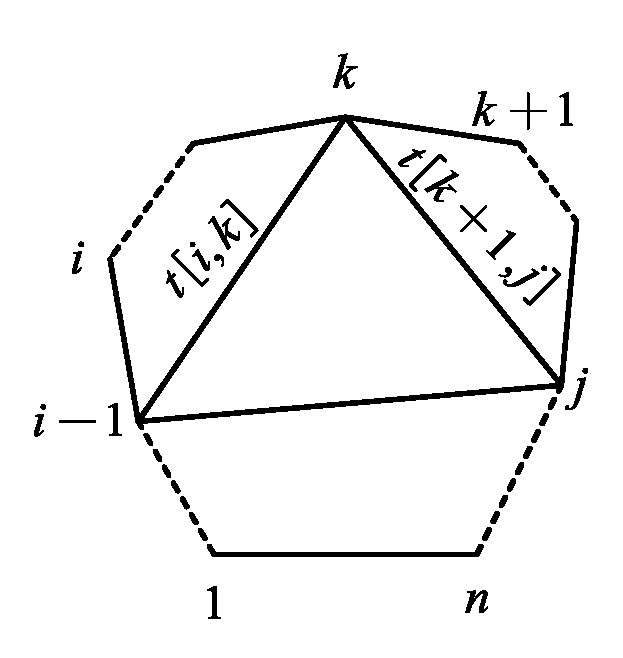
\includegraphics[width=0.25\textwidth]{images/title/子问题归约.pdf}
		\caption{子问题归约图}
		\label{fig:子问题归约}
	\end{figure}
	考虑子问题$A[i,j]$的划分, 假设它的所有划分方案中最小权值为$t[i,j]$. 从$i,i+1,\cdots,j-1$中任选顶点$k$, 它与底边$(i-1)j$构成一个三角形(图\ref{fig:子问题归约}中的三角形). 这个三角形将$A[i,j]$划分成两个凸多边形: $A[i,k]$和$A[k+1,j]$, 从而产生了两个子问题. 这两个凸多边形的划分方案的最小权值分别为$t[i,k]$和$t[k+1,j]$. 根据DP思想, $A[i,j]$相对于这个顶点$k$的划分方案的最小权值是
	$$
	t\left[ i,k \right] +t\left[ k+1,j \right] +d_{\left( i-1 \right) k}+d_{kj}+d_{\left( i-1 \right) j}
	$$
	其中$d_{\left( i-1 \right) k}+d_{kj}+d_{\left( i-1 \right) j}$是三角形$(i-1)kj$的周长, 于是得到递推关系
	$$
	t\left[ i,j \right] =\begin{cases}
		0,&		i=j\\
		\underset{i\le k\le j-1}{\text{min}}\left\{ t\left[ i,k \right] +t\left[ k+1,j \right] +d_{\left( i-1 \right) k}+d_{kj}+d_{\left( i-1 \right) j} \right\} ,&		i<j\\
	\end{cases}
	$$
	根据上述递推关系可知, 若最优划分$t[i,j]$与$(i-1)j$相连的三角形第三顶是$k$, 则这个划分也是$A[i,k]$和$A[k+1,j]$的最优划分, 即最优子结构性质得证. 可以通过标记函数来得到最小权值对应顶点$k$的位置, 于是该划分算法最坏情况下的时间复杂度为$O\left( n^3 \right)$.
\begin{tcblisting}{listing engine=minted,boxrule=0.1mm,
colback=blue!5!white,colframe=blue!75!black,
listing only,left=5mm,enhanced,sharp corners=all,
overlay={\begin{tcbclipinterior}\fill[red!20!blue!20!white] (frame.south west)
rectangle ([xshift=5mm]frame.north west);\end{tcbclipinterior}},
minted language=c++,
minted style=tango,
minted options={fontsize=\small,breaklines,autogobble,linenos,numbersep=3mm}}
void MatrixChain(int **d, int n, int **t, int **s) {
    for (int i = 1; i <= n; i++) t[i][i] = 0;
    for (int r = 2; r <= n; r++){
        for (int i = 1; i <= n - r + 1; i++){
            int j = i + r - 1;
            t[i][j] = t[i + 1][j] + d[i - 1][i] + d[i][j] + d[i - 1][j];
            s[i][j] = i;
            for (int k = i + 1; k < j; k++){
                int T = t[i][k] + t[k + 1][j] + d[i - 1][k] + d[k][j] + d[i - 1][j];
                if(t < t[i][j]) {
                    t[i][j] = t, s[i][j] = k; 
                }
            }
        }
    }
}
\end{tcblisting}
\end{homeworkProblem}



% 引用文献
\bibliographystyle{unsrt}  % unsrt:根据引用顺序编号
\bibliography{refs}


\end{document}
